% Gabarit pandoc des corrigés publiés (brut et guidé). Contenu sans marque ni nom de site.
% Compilation : lualatex (latexmk -lualatex).
% Le Markdown reste la source unique : ne pas éditer ce fichier .tex à la main.
\documentclass[11pt,a4paper]{article}

% --- Moteur, polices (Latin Modern) et langue ---------------------------------
\usepackage{iftex}
\ifLuaTeX\else\errmessage{Ce document se compile avec lualatex}\fi
\usepackage{amsmath,amssymb,mathtools}
\usepackage{fontspec}
% mathrm=sym : \mathrm prend ses glyphes dans la police mathématique (ℓ, μ, Ω), comme KaTeX.
\usepackage[math-style=TeX,bold-style=TeX,mathrm=sym]{unicode-math}
% Repli pour les glyphes absents de Latin Modern (indices et exposants Unicode,
% flèches, filets des schémas en texte, symboles) : DejaVu, puis Latin Modern Math
% (ℓ, lettres mathématiques Unicode des légendes).
\directlua{
  luaotfload.add_fallback("repliTexte", {"DejaVuSerif:mode=harf;", "DejaVuSans:mode=harf;", "file:latinmodern-math.otf:mode=harf;"})
  luaotfload.add_fallback("repliMono", {"DejaVuSansMono:mode=harf;", "DejaVuSans:mode=harf;", "file:latinmodern-math.otf:mode=harf;"})
}
\setmainfont{Latin Modern Roman}[RawFeature={fallback=repliTexte}]
\setsansfont{Latin Modern Sans}[RawFeature={fallback=repliTexte}]
\setmonofont{Latin Modern Mono}[RawFeature={fallback=repliMono}]
\setmathfont{Latin Modern Math}
\usepackage[french]{babel}
\frenchsetup{SmallCapsFigTabCaptions=false}

% --- Mise en page --------------------------------------------------------------
\usepackage[a4paper,margin=2.2cm,headheight=14pt,footskip=1.2cm]{geometry}
\usepackage{microtype}
\setlength{\emergencystretch}{4em}
\tolerance=1500
\setlength{\parindent}{0pt}
\setlength{\parskip}{0.55\baselineskip plus 2pt minus 1pt}
\usepackage{xcolor}
% Gris nommés : babel-french rend « ! » actif dans le document.
\definecolor{gris2}{gray}{0.98}
\definecolor{gris3}{gray}{0.97}
\definecolor{gris5}{gray}{0.95}
\definecolor{gris35}{gray}{0.65}
\definecolor{gris40}{gray}{0.60}
\definecolor{gris45}{gray}{0.55}
\definecolor{gris50}{gray}{0.50}
\definecolor{gris55}{gray}{0.45}
\definecolor{gris60}{gray}{0.40}
\definecolor{gris65}{gray}{0.35}
\definecolor{gris70}{gray}{0.30}
\definecolor{gris80}{gray}{0.20}
\definecolor{gris85}{gray}{0.15}
\usepackage{graphicx}
\usepackage{float}
\usepackage{caption}
\captionsetup{font=small,labelformat=empty,justification=centering}
\usepackage{booktabs,longtable,array,multirow,calc}
\usepackage{siunitx}
\sisetup{locale=FR}
\usepackage[version=4]{mhchem}
\usepackage{listings}
\usepackage{fancyhdr}
\usepackage{lastpage}
\usepackage[most]{tcolorbox}
\usepackage{enumitem}
\setlist{nosep,leftmargin=*,topsep=2pt}
\usepackage[hidelinks,unicode]{hyperref}
\usepackage{bookmark}
\hypersetup{pdftitle={Centrale-Supélec PSI — Mathématiques 1 2026 · Corrigé},pdfauthor={Rédigé par IA},pdfcreator={LaTeX},pdfsubject={Corrigé brut}}
\usepackage{xurl}

% --- Pandoc : listes, tableaux, figures ----------------------------------------
\providecommand{\passthrough}[1]{#1}
\providecommand{\tightlist}{\setlength{\itemsep}{0pt}\setlength{\parskip}{0pt}}

\makeatletter
\def\maxwidth{\ifdim\Gin@nat@width>\linewidth\linewidth\else\Gin@nat@width\fi}
\def\maxheight{\ifdim\Gin@nat@height>0.55\textheight 0.55\textheight\else\Gin@nat@height\fi}
\makeatother
\setkeys{Gin}{width=\maxwidth,height=\maxheight,keepaspectratio}
\setcounter{secnumdepth}{-\maxdimen}
\providecommand{\pandocbounded}[1]{#1}

% --- Code (listings) -----------------------------------------------------------
\lstset{
  basicstyle=\ttfamily\small,
  columns=fullflexible,
  keepspaces=true,
  breaklines=true,
  breakatwhitespace=false,
  postbreak=\mbox{\textcolor{gris50}{$\hookrightarrow$}\space},
  frame=single,
  rulecolor=\color{gris35},
  framesep=4pt,
  xleftmargin=5pt,xrightmargin=5pt,
  backgroundcolor=\color{gris3},
  keywordstyle=\bfseries,
  commentstyle=\color{gris65},
  stringstyle=\color{gris80},
  showstringspaces=false,
  tabsize=4,
  extendedchars=true,
  aboveskip=6pt,belowskip=6pt,
}

% --- Macros des corrigés (KaTeX ↔ LaTeX) ---------------------------------------
% Les corrigés sont écrits pour KaTeX : on définit ici ce que KaTeX connaît et
% que LaTeX n'a pas, sans jamais retoucher le Markdown.
\providecommand{\R}{\mathbb{R}}
\providecommand{\N}{\mathbb{N}}
\providecommand{\Z}{\mathbb{Z}}
\providecommand{\Q}{\mathbb{Q}}
\providecommand{\C}{\mathbb{C}}
\providecommand{\dd}{\mathrm{d}}
\providecommand{\llbracket}{\lBrack}
\providecommand{\rrbracket}{\rBrack}
\providecommand{\lBrace}{\lbrace}
\providecommand{\rBrace}{\rbrace}
\providecommand{\Box}{\square}
\providecommand{\Diamond}{\lozenge}
\providecommand{\varnothing}{\emptyset}
\providecommand{\argmax}{\operatorname*{arg\,max}}
\providecommand{\argmin}{\operatorname*{arg\,min}}
\renewcommand{\leq}{\leqslant}
\renewcommand{\geq}{\geqslant}

% Équation hors texte : réduite à la largeur de la ligne si elle déborde.
\newsavebox{\boiteequation}
\newcommand{\equationajustee}[1]{%
  \sbox{\boiteequation}{$\displaystyle #1$}%
  \ifdim\wd\boiteequation>\linewidth
    \[\resizebox{\linewidth}{!}{\usebox{\boiteequation}}\]%
  \else
    \[#1\]%
  \fi}

% --- Encadrés pédagogiques (sobres, lisibles en noir et blanc) -----------------
\tcbset{
  encadre/.style={
    enhanced,breakable,sharp corners,
    colback=white,colframe=gris55,
    boxrule=0.4pt,leftrule=2.2pt,
    left=6pt,right=6pt,top=3pt,bottom=3pt,
    before skip=6pt,after skip=6pt,
    fonttitle=\bfseries\small,coltitle=black,
    attach title to upper,after title={\quad},
    parbox=false,
  }
}
\newtcolorbox{indication}[1]{encadre,colframe=gris45,colback=gris2,title={Indication~#1}}
\newtcolorbox{methode}{encadre,colframe=gris70,title={Méthode}}
\newtcolorbox{piege}{encadre,colframe=gris85,boxrule=0.8pt,leftrule=2.2pt,title={Piège}}
\newtcolorbox{jury}{encadre,colframe=gris60,colback=gris5,title={Jury}}
\newtcolorbox{encadrenote}{encadre,colframe=gris40}

% --- Titres de section ---------------------------------------------------------
\usepackage{titlesec}
\titleformat{\section}{\Large\bfseries}{}{0pt}{}
\titleformat{\subsection}{\large\bfseries}{}{0pt}{}
\titleformat{\subsubsection}{\normalsize\bfseries}{}{0pt}{}
\titlespacing*{\section}{0pt}{14pt plus 4pt minus 2pt}{6pt}
\titlespacing*{\subsection}{0pt}{10pt plus 3pt minus 2pt}{4pt}
\titlespacing*{\subsubsection}{0pt}{8pt plus 2pt minus 2pt}{2pt}

% --- En-tête et pied de page ---------------------------------------------------
\pagestyle{fancy}
\fancyhf{}
\fancyhead[L]{\small\textsc{Corrigé brut} · Centrale-Supélec PSI}
\fancyhead[R]{\small Maths 1 2026}
\fancyfoot[L]{\footnotesize Corrigé rédigé par IA, non officiel}
\fancyfoot[R]{\footnotesize \thepage\,/\,\pageref*{LastPage}}
\renewcommand{\headrulewidth}{0.4pt}
\renewcommand{\footrulewidth}{0pt}
\fancypagestyle{plain}{\fancyhf{}\fancyfoot[R]{\footnotesize \thepage\,/\,\pageref*{LastPage}}\fancyfoot[L]{\footnotesize Corrigé rédigé par IA, non officiel}\renewcommand{\headrulewidth}{0pt}}

\begin{document}
\thispagestyle{plain}
\begin{center}
  {\small\scshape Corrigé brut}\par\smallskip
  {\LARGE\bfseries Centrale-Supélec PSI — Mathématiques 1 2026 · Corrigé\par}\medskip
  {\large Centrale-Supélec · PSI · Maths 1 · 2026\par}
\end{center}
\vspace{2pt}\hrule\vspace{8pt}

\emph{Corrigé rédigé par IA, non officiel. Signalez toute erreur.}

Notations : \(P_i\) (resp. \(F_i\)) désigne l'événement « le \(i\)-ième lancer donne pile (resp. face) ». Les lancers sont mutuellement indépendants, de même loi, et \(p+q=1\).

\hypertarget{a-les-cas-ouxf9-n1-et-n2}{%
\section{\texorpdfstring{A --- Les cas où \(n=1\) et \(n=2\)}{A --- Les cas où n=1 et n=2}}\label{a-les-cas-ouxf9-n1-et-n2}}

\hypertarget{i-le-cas-ouxf9-n1}{%
\subsection{\texorpdfstring{I --- Le cas où \(n=1\)}{I --- Le cas où n=1}}\label{i-le-cas-ouxf9-n1}}

\hypertarget{question-1}{%
\subsection{Question 1}\label{question-1}}

Soit \(k\in{\mathbb{N}}^*\). On a
\equationajustee{(X_1=k)=F_1\cap\dots\cap F_{k-1}\cap P_k,}
donc par indépendance \(P(X_1=k)=q^{k-1}p\). Comme
\equationajustee{\sum_{k\geqslant1}q^{k-1}p=\frac{p}{1-q}=1,}
on obtient
\equationajustee{\begin{aligned}
P(X_1=+\infty)&=1-\sum_{k\geqslant1}P(X_1=k)\\
&=0.
\end{aligned}}

\equationajustee{\boxed{\begin{aligned}{}&\forall k\in{\mathbb{N}}^*,\ P(X_1=k)=q^{k-1}p,\\
&P(X_1=+\infty)=0 :\ X_1\sim\mathcal{G}(p).
\end{aligned}}}

\hypertarget{question-2}{%
\subsection{Question 2}\label{question-2}}

Pour une loi géométrique de paramètre \(p\) :

\equationajustee{\boxed{\begin{aligned}
G_{X_1}(z)&=\frac{pz}{1-qz}\quad(|z|<1/q),\\
E(X_1)&=\frac1p,\\
V(X_1)&=\frac{q}{p^2}.
\end{aligned}}}

\hypertarget{question-3}{%
\subsection{Question 3}\label{question-3}}

\emph{Fonction génératrice.} Soit \(|z|<1/q\). La série \(\sum_{k\geqslant1}q^{k-1}pz^k\) est géométrique de raison \(qz\), avec \(|qz|<1\) ; elle converge donc absolument et
\equationajustee{G_{X_1}(z)=pz\sum_{k\geqslant1}(qz)^{k-1}=\frac{pz}{1-qz}.}
Le rayon de convergence vaut \(1/q>1\).

\emph{Moments.} Le rayon \(1/q\) est strictement supérieur à \(1\). Les séries dérivées \(\sum kP(X_1=k)z^{k-1}\) et \(\sum k(k-1)P(X_1=k)z^{k-2}\) ont le même rayon, donc convergent absolument en \(z=1\).

Ainsi \(X_1\) admet un moment d'ordre 2, avec
\equationajustee{\begin{aligned}
E(X_1)&=G'_{X_1}(1),\\
E(X_1(X_1-1))&=G''_{X_1}(1).
\end{aligned}}
Or
\equationajustee{\begin{aligned}
G'_{X_1}(z)&=\frac{p}{(1-qz)^2},\\
G''_{X_1}(z)&=\frac{2pq}{(1-qz)^3},
\end{aligned}}
d'où \(E(X_1)=\frac{p}{p^2}=\frac1p\) et \(E(X_1(X_1-1))=\frac{2q}{p^2}\). Par la formule de König-Huygens,
\equationajustee{\begin{aligned}
V(X_1)&=G''(1)+G'(1)-G'(1)^2\\
&=\frac{2q}{p^2}+\frac1p-\frac1{p^2}\\
&=\frac{2q+p-1}{p^2}\\
&=\frac{q}{p^2}.
\end{aligned}}

\hypertarget{ii-le-cas-ouxf9-n2}{%
\subsection{\texorpdfstring{II --- Le cas où \(n=2\)}{II --- Le cas où n=2}}\label{ii-le-cas-ouxf9-n2}}

\hypertarget{question-4}{%
\subsection{Question 4}\label{question-4}}

\((X_2=1)\) est impossible (un seul lancer ne peut contenir deux piles), et \((X_2=2)=P_1\cap P_2\). Donc
\equationajustee{\boxed{\begin{aligned}
P(X_2=1)&=0,\\
P(X_2=2)&=p^2.
\end{aligned}}}

\hypertarget{question-5}{%
\subsection{Question 5}\label{question-5}}

Soit \(k>2\) et supposons \(X_2=k\). Les deux premiers lancers ne donnent pas \(PP\), sinon on aurait \(X_2=2\). Donc \textbf{les deux premiers résultats appartiennent à \(\{FF,FP,PF\}\)} : soit le premier lancer donne face, soit les deux premiers donnent \(PF\).

Plus précisément, fixons \(k\). L'événement \((X_2=k)\) impose \(P_{k-1}\cap P_k\). Si \(k\geqslant3\), il impose aussi \(F_{k-2}\) :
- \(k=3\) : \(F_1P_2P_3\), l'ensemble est \(\{FP\}\) ;
- \(k=4\) : \(F_2P_3P_4\), donc le lancer 2 est face. L'ensemble est \(\{FF,PF\}\) (suites \(FFPP\) et \(PFPP\)) ;
- \(k\geqslant5\) : les trois issues sont possibles. On place \(k-4\geqslant1\) faces au milieu. Par exemple : \(FF\,F\cdots F\,PP\), \(FP\,F\cdots F\,PP\), \(PF\,F\cdots F\,PP\).

\hypertarget{question-6}{%
\subsection{Question 6}\label{question-6}}

Considérons les événements \(F_1\), \(P_1\cap F_2\) et \(P_1\cap P_2\). Ils sont deux à deux incompatibles, de réunion \(\Omega\).

Leurs probabilités \(q\), \(pq\), \(p^2\) sont non nulles : c'est un système complet. Soit \(k>2\).

\begin{itemize}
\tightlist
\item
  Sur \(P_1\cap P_2\), \(X_2=2\neq k\) : \(P(X_2=k\cap P_1\cap P_2)=0\).
\item
  Sur \(F_1\), aucune série de deux piles ne contient le lancer 1. Ainsi \(X_2=k\) équivaut à : la première série \(PP\) des lancers à partir du deuxième se termine au rang \(k-1\) de cette suite. Ces lancers sont indépendants, de même loi, et indépendants du premier, donc \(P(F_1\cap(X_2=k))=q\,P(X_2=k-1)\).
\item
  Sur \(P_1\cap F_2\), aucune série \(PP\) ne contient les lancers 1 ou 2. De même, \(P(P_1\cap F_2\cap(X_2=k))=pq\,P(X_2=k-2)\), avec \(k-2\geqslant1\).
\end{itemize}

\begin{figure}[H]
\centering
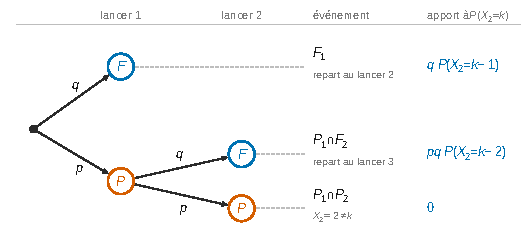
\includegraphics{figures/q6-arbre-systeme-complet.pdf}
\caption*{Figure 1 --- Arbre des deux premiers lancers pour n = 2 : le système
complet F₁, P₁ ∩ F₂, P₁ ∩ P₂ et l'apport de chaque événement à P(X₂ =
k), pour k \textgreater{} 2}
\end{figure}

La formule des probabilités totales donne
\equationajustee{\boxed{\begin{aligned}
\forall k>2,\quad P(X_2=k)&=q\,P(X_2=k-1)\\
&\quad+pq\,P(X_2=k-2).
\end{aligned}}}

\hypertarget{question-7}{%
\subsection{Question 7}\label{question-7}}

Soit \(T=X^2-qX-pq\). Son discriminant \(\Delta=q^2+4pq\) est strictement positif : \(T\) a deux racines réelles
\equationajustee{\begin{aligned}
r_1&=\frac{q+\sqrt{q^2+4pq}}{2},\\
r_2&=\frac{q-\sqrt{q^2+4pq}}{2},
\end{aligned}}
avec \(r_2<r_1\).

Leur produit vaut \(-pq<0\), donc \(r_2<0<r_1\). Leur somme vaut \(q>0\), d'où
\equationajustee{|r_1|-|r_2|=r_1+r_2=q>0,}
soit \(|r_2|<|r_1|\).

Enfin, on évalue le trinôme en \(1\), \(-1\) et \(0\) :
\equationajustee{\begin{aligned}
T(1)&=1-q-pq\\
&=p-pq\\
&=p^2>0,\\
T(-1)&=1+q-pq\\
&=1+q^2>0,\\
T(0)&=-pq<0.
\end{aligned}}
Par le théorème des valeurs intermédiaires, \(T\) s'annule dans \(]-1,0[\) et dans \(]0,1[\). Ces deux zéros sont \(r_2\) et \(r_1\), donc
\equationajustee{\boxed{\begin{aligned}{}&-1<r_2<0<r_1<1,\\
&|r_2|<|r_1|.
\end{aligned}}}

\begin{figure}[H]
\centering
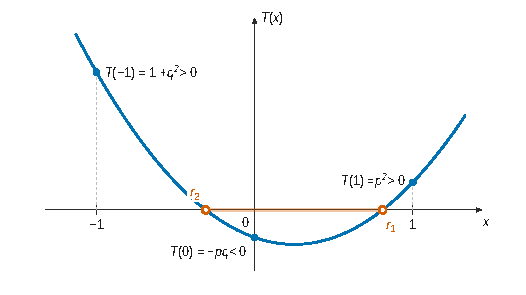
\includegraphics{figures/q7-trinome-racines.pdf}
\caption*{Figure 2 --- Allure du trinôme X² − qX − pq, tracé pour p = q = 1/2 :
positif en −1 et en 1, négatif en 0, il a une racine r₂ entre −1 et 0 et
une racine r₁ entre 0 et 1}
\end{figure}

\hypertarget{question-8}{%
\subsection{Question 8}\label{question-8}}

La série \(\sum r_1^{k-1}z^k\) est géométrique, de rayon \(1/r_1\). De même, \(\sum r_2^{k-1}z^k\) a pour rayon \(1/|r_2|\). Ces rayons sont distincts puisque \(|r_2|<r_1\), donc le rayon de la différence est le plus petit des deux :
\equationajustee{\boxed{R=\frac1{r_1}>1.}}

\hypertarget{question-9}{%
\subsection{Question 9}\label{question-9}}

D'après Q6, \(u_k=P(X_2=k)\) vérifie, pour \(k\geqslant3\),
\equationajustee{u_k=qu_{k-1}+pqu_{k-2}.}
L'équation caractéristique \(x^2-qx-pq=0\) a deux racines réelles distinctes \(r_1,r_2\). Il existe donc \((\alpha,\beta)\in{\mathbb{R}}^2\) tels que, pour tout \(k\geqslant1\),
\equationajustee{u_k=\alpha r_1^{k}+\beta r_2^{k}.}
Les conditions \(u_1=0\) et \(u_2=p^2\) donnent
\equationajustee{\begin{aligned}
\alpha r_1+\beta r_2&=0,\\
\alpha r_1^2+\beta r_2^2&=p^2,
\end{aligned}}
d'où \(\alpha r_1(r_1-r_2)=p^2\), puis
\equationajustee{\begin{aligned}
\alpha&=\frac{p^2}{r_1(r_1-r_2)},\\
\beta&=-\frac{p^2}{r_2(r_1-r_2)}.
\end{aligned}}
Ainsi, avec \(r_1-r_2=\sqrt{q^2+4pq}\), pour tout \(k\geqslant2\) (et même \(k\geqslant1\)) :
\equationajustee{\boxed{P(X_2=k)=\frac{p^2}{\sqrt{q^2+4pq}}\left(r_1^{k-1}-r_2^{k-1}\right).}}

\hypertarget{question-10}{%
\subsection{Question 10}\label{question-10}}

\(X_2\) prend la valeur \(+\infty\) si et seulement si elle est supérieure ou égale à tout entier :
\equationajustee{\boxed{(X_2=+\infty)=\bigcap_{k\in{\mathbb{N}}^*}(X_2\geqslant k).}}
La suite \(\big((X_2\geqslant k)\big)_k\) est décroissante pour l'inclusion ; par continuité décroissante,
\equationajustee{\begin{aligned}
P(X_2=+\infty)&=\lim_{k\to+\infty}P(X_2\geqslant k)\\
&=\lim_{k\to+\infty}\Big(1-\sum_{j=1}^{k-1}P(X_2=j)\Big)\\
&=1-\sum_{j=1}^{+\infty}P(X_2=j).
\end{aligned}}
Comme \(|r_1|,|r_2|<1\), d'après Q9,
\equationajustee{\begin{aligned}
\sum_{j\geqslant1}P(X_2=j)&=\frac{p^2}{r_1-r_2}\left(\frac1{1-r_1}-\frac1{1-r_2}\right)\\
&=\frac{p^2}{(1-r_1)(1-r_2)}\\
&=\frac{p^2}{T(1)}\\
&=1,
\end{aligned}}
car \((1-r_1)(1-r_2)=T(1)=p^2\). Donc
\equationajustee{\boxed{P(X_2=+\infty)=0.}}

\hypertarget{question-11}{%
\subsection{Question 11}\label{question-11}}

Soit \(|z|<R=1/r_1\) ; alors \(|r_2z|<|r_1z|<1\). D'après Q9 et Q10, \(G_{X_2}(z)=\sum_{k\geqslant1}P(X_2=k)z^k\) et
\equationajustee{\begin{aligned}
G_{X_2}(z)&=\frac{p^2}{r_1-r_2}\sum_{k\geqslant2}\left(r_1^{k-1}-r_2^{k-1}\right)z^k\\
&=\frac{p^2z^2}{r_1-r_2}\left(\frac{r_1}{1-r_1z}-\frac{r_2}{1-r_2z}\right)\\
&=\frac{p^2z^2}{(1-r_1z)(1-r_2z)}.
\end{aligned}}
Or
\equationajustee{\begin{aligned}
(1-r_1z)(1-r_2z)&=1-(r_1+r_2)z+r_1r_2z^2\\
&=1-qz-pqz^2,
\end{aligned}}
donc
\equationajustee{\boxed{\forall z\in\mathbb{C},\ |z|<R,\quad G_{X_2}(z)=\frac{p^2z^2}{1-qz-pqz^2}.}}

\hypertarget{question-12}{%
\subsection{Question 12}\label{question-12}}

La série entière \(\sum P(X_2=k)z^k\) a pour rayon \(R=1/r_1>1\). Ses séries dérivées première et seconde ont le même rayon, donc convergent absolument en \(z=1\).

Ainsi \(\sum kP(X_2=k)\) et \(\sum k(k-1)P(X_2=k)\) convergent, donc aussi \(\sum k^2P(X_2=k)\).

Comme \(X_2\) est presque sûrement finie (Q10), \textbf{\(X_2\) admet une espérance et une variance}, avec
\equationajustee{\begin{aligned}
E(X_2)&=G'(1),\\
E(X_2(X_2-1))&=G''(1).
\end{aligned}}

\hypertarget{question-13}{%
\subsection{Question 13}\label{question-13}}

Notons \(G=G_{X_2}\) et \(D(z)=1-qz-pqz^2\). On a \(D(z)G(z)=p^2z^2\) sur \(]-R,R[\), intervalle contenant \(1\). De plus :
\equationajustee{\begin{aligned}
G(1)&=1,\\
D(1)&=p^2,\\
D'(1)&=-q-2pq\\
&=-q(1+2p),\\
D''&=-2pq.
\end{aligned}}

En dérivant une fois en \(1\) :
\equationajustee{D'(1)+p^2G'(1)=2p^2,}
d'où
\equationajustee{\begin{aligned}
p^2G'(1)&=2p^2+(1-p)(1+2p)\\
&=1+p,
\end{aligned}}
et
\equationajustee{\boxed{E(X_2)=\frac{1+p}{p^2}=\frac1{p^2}+\frac1p.}}
En dérivant deux fois en \(1\) :
\equationajustee{D''(1)+2D'(1)G'(1)+p^2G''(1)=2p^2,}
donc
\equationajustee{\begin{aligned}
p^2G''(1)&=2p^2+2pq+2q(1+2p)\frac{1+p}{p^2}\\
&=2p+\frac{2(1+2p-p^2-2p^3)}{p^2},
\end{aligned}}
puisque \((1-p)(1+2p)(1+p)=1+2p-p^2-2p^3\).

Posons \(u=1/p\). Alors \(G''(1)=2u^4+4u^3-2u^2-2u\) et \(E(X_2)=u^2+u\), donc
\equationajustee{\begin{aligned}
V(X_2)&=G''(1)+G'(1)-G'(1)^2\\
&=(2u^4+4u^3-2u^2-2u)+(u^2+u)-(u^4+2u^3+u^2)\\
&=u^4+2u^3-2u^2-u,
\end{aligned}}
\equationajustee{\boxed{V(X_2)=\frac1{p^4}+\frac2{p^3}-\frac2{p^2}-\frac1p.}}
(Contrôle : pour \(p=\frac12\), \(E(X_2)=6\) et \(V(X_2)=22\).)

\hypertarget{b-le-cas-ouxf9-n3}{%
\section{\texorpdfstring{B --- Le cas où \(n=3\)}{B --- Le cas où n=3}}\label{b-le-cas-ouxf9-n3}}

\hypertarget{i-uxe9tude-guxe9nuxe9rale-uxe0-laide-de-lalguxe8bre-linuxe9aire}{%
\subsection{I --- Étude générale à l'aide de l'algèbre linéaire}\label{i-uxe9tude-guxe9nuxe9rale-uxe0-laide-de-lalguxe8bre-linuxe9aire}}

\hypertarget{question-14}{%
\subsection{Question 14}\label{question-14}}

Trois piles consécutifs demandent au moins trois lancers, et \((X_3=3)=P_1\cap P_2\cap P_3\) :
\equationajustee{\boxed{\begin{aligned}
P(X_3=1)&=0,\\
P(X_3=2)&=0,\\
P(X_3=3)&=p^3.
\end{aligned}}}

\hypertarget{question-15}{%
\subsection{Question 15}\label{question-15}}

Considérons les événements
\equationajustee{\begin{aligned}
E_1&=F_1,\\
E_2&=P_1\cap F_2,\\
E_3&=P_1\cap P_2\cap F_3,\\
E_0&=P_1\cap P_2\cap P_3.
\end{aligned}}
Ils forment un système complet (classement selon le rang du premier face parmi les trois premiers lancers). Leurs probabilités respectives sont
\equationajustee{q,\qquad pq,\qquad p^2q,\qquad p^3.}

Soit \(k>3\). Sur \(E_0\), \(X_3=3\neq k\).

Soit \(i\in\{1,2,3\}\). Sur \(E_i\), le face du rang \(i\) empêche toute série de trois piles de contenir un lancer de rang \(\leqslant i\).

Le processus recommence au lancer \(i+1\), avec des lancers indépendants de même loi et indépendants des \(i\) premiers. D'où \(P(E_i\cap(X_3=k))=P(E_i)P(X_3=k-i)\), avec \(k-i\geqslant1\).

Par la formule des probabilités totales :
\equationajustee{\boxed{\begin{aligned}
\forall k>3,\quad P(X_3=k)&=qP(X_3=k-1)+pqP(X_3=k-2)\\
&\quad+qp^2P(X_3=k-3).
\end{aligned}}}

\hypertarget{question-16}{%
\subsection{Question 16}\label{question-16}}

Soit \(k\geqslant1\). Comme \(k+3>3\), Q15 donne la première composante de \(U_{k+1}\). Les deux autres sont les deux premières de \(U_k\) :
\equationajustee{\boxed{M=\begin{pmatrix}q&pq&qp^2\\1&0&0\\0&1&0\end{pmatrix}.}}

\hypertarget{question-17}{%
\subsection{Question 17}\label{question-17}}

En développant \(\det(XI_3-M)\) selon la première colonne :
\equationajustee{\begin{aligned}
\chi_M(X)&=\begin{vmatrix}X-q&-pq&-qp^2\\-1&X&0\\0&-1&X\end{vmatrix}\\
&=(X-q)X^2+\begin{vmatrix}-pq&-qp^2\\-1&X\end{vmatrix},
\end{aligned}}
\equationajustee{\boxed{\chi_M(X)=X^3-qX^2-pqX-qp^2.}}

\hypertarget{question-18}{%
\subsection{Question 18}\label{question-18}}

On a \(\chi_M(0)=-qp^2<0\) et
\equationajustee{\begin{aligned}
\chi_M(1)&=1-q(1+p+p^2)\\
&=1-(1-p^3)\\
&=p^3>0.
\end{aligned}}
Par le théorème des valeurs intermédiaires, \(\chi_M\) s'annule sur \(]0,1[\).

\emph{Unicité.} Pour \(x>0\), on a
\equationajustee{\frac{\chi_M(x)}{x^3}=1-\frac qx-\frac{pq}{x^2}-\frac{qp^2}{x^3}.}
Cette fonction est strictement croissante sur \(]0,+\infty[\), donc \(\chi_M\) s'annule au plus une fois sur \(]0,+\infty[\).

Ainsi \textbf{\(\chi_M\) a une unique racine \(\lambda_1\) dans \(]0,1[\)}, c'est sa seule racine positive, et
\equationajustee{\begin{aligned}
\chi_M&<0\ \text{sur}\ ]0,\lambda_1[,\\
\chi_M&>0\ \text{sur}\ ]\lambda_1,+\infty[.
\end{aligned}}

\hypertarget{question-19}{%
\subsection{Question 19}\label{question-19}}

\equationajustee{\begin{aligned}
(X-p)\chi_M(X)&=X^4-qX^3-pqX^2-qp^2X\\
&\quad-pX^3+pqX^2+qp^2X+qp^3\\
&=X^4-(p+q)X^3+qp^3\\
&=X^4-X^3+qp^3.
\end{aligned}}

Soit \(\psi=X^4-X^3+qp^3\). Alors \(\psi'=X^2(4X-3)\).

Ainsi \(\psi\) est strictement décroissante sur \(]-\infty,\frac34]\) et strictement croissante sur \([\frac34,+\infty[\) : elle a au plus deux racines réelles distinctes. De plus \(\psi(p)=p^3(p-1+q)=0\).

On calcule aussi
\equationajustee{\chi_M(p)=p^2(p-3q).}

\emph{Cas \(\psi(\frac34)<0\).} Alors \(\psi\) a exactement deux racines réelles, simples. L'une est \(p\). L'autre est \(\lambda_1\) : toute racine de \(\chi_M\) est racine de \(\psi\).

Supposons \(\lambda_1=p\). Alors \(\chi_M(p)=0\), ce qui donne \(p^2(p-3q)=0\), soit \(p=\frac34\). On aurait alors \(\psi(\frac34)=\psi(p)=0\) : contradiction.

Les racines réelles de \(\chi_M\) sont parmi \(\{p,\lambda_1\}\), et \(\chi_M(p)\neq0\). Donc \textbf{\(\lambda_1\) est la seule racine réelle de \(\chi_M\)}.

\emph{Cas \(\psi(\frac34)=0\).} Comme \(\psi\geqslant\psi(\frac34)\) et \(\psi(p)=0\), cela impose \(p=\frac34\).

Alors \(\frac34\) est l'unique racine réelle de \(\psi\), donc de \(\chi_M\). Ainsi \(\lambda_1=\frac34\).

\emph{Cas \(\psi(\frac34)>0\).} Il est exclu puisque \(\psi(p)=0\).

Dans tous les cas, \(\chi_M\) admet une seule racine réelle, \(\lambda_1\).

\hypertarget{question-20}{%
\subsection{Question 20}\label{question-20}}

\(\chi_M\), réel de degré 3, est scindé sur \(\mathbb{C}\). Sa seule racine réelle est \(\lambda_1\). Ses deux autres racines sont donc non réelles et conjuguées, \(\lambda_2\) et \(\overline{\lambda_2}\), avec \(\lambda_2\neq\overline{\lambda_2}\).

Les trois racines \(\lambda_1,\lambda_2,\overline{\lambda_2}\) sont deux à deux distinctes. Ainsi \(M\in{\mathcal{M}}_3(\mathbb{C})\) a trois valeurs propres distinctes, donc \textbf{\(M\) est diagonalisable dans \(\mathbb{C}\)}.

\hypertarget{question-21}{%
\subsection{Question 21}\label{question-21}}

Par récurrence, \(U_k=M^{k-1}U_1\) pour \(k\geqslant1\). De plus \(M^{k-1}=QD^{k-1}Q^{-1}\), avec \(D=\mathrm{diag}(\lambda_1,\lambda_2,\overline{\lambda_2})\).

Posons \(V=Q^{-1}U_1=(v_1,v_2,v_3)^\top\), et notons \((w_1,w_2,w_3)\) la troisième ligne de \(Q\). La troisième composante de \(U_k\) vaut alors
\equationajustee{P(X_3=k)=w_1v_1\lambda_1^{k-1}+w_2v_2\lambda_2^{k-1}+w_3v_3\overline{\lambda_2}^{\,k-1}.}
Posons
\equationajustee{\begin{aligned}
A&=w_1v_1,\\
B&=w_2v_2,\\
C&=w_3v_3,
\end{aligned}}
indépendants de \(k\). Pour tout \(k\geqslant1\) :
\equationajustee{\boxed{P(X_3=k)=A\lambda_1^{k-1}+B\lambda_2^{k-1}+C\overline{\lambda_2}^{\,k-1},}}
avec \(\lambda_1\in]0,1[\) (Q18) et \(\lambda_2\in\mathbb{C}\).

\hypertarget{question-22}{%
\subsection{Question 22}\label{question-22}}

Pour \(k=1,2,3\) (Q14) :
\equationajustee{\begin{aligned}
A+B+C&=0,\\
A\lambda_1+B\lambda_2+C\overline{\lambda_2}&=0,\\
A\lambda_1^2+B\lambda_2^2+C\overline{\lambda_2}^2&=p^3.
\end{aligned}}
Soit \(L(X)=(X-\lambda_2)(X-\overline{\lambda_2})=X^2-sX+m\), avec \(s=2\mathrm{Re}\lambda_2\) et \(m=|\lambda_2|^2\).

La combinaison (troisième) \(-s\,\)(deuxième) \(+m\,\)(première) donne
\equationajustee{A\,L(\lambda_1)+B\,L(\lambda_2)+C\,L(\overline{\lambda_2})=p^3,}
soit
\equationajustee{A\,L(\lambda_1)=p^3.}
Comme \(L(\lambda_1)=(\lambda_1-\lambda_2)(\lambda_1-\overline{\lambda_2})=|\lambda_1-\lambda_2|^2\neq0\) :
\equationajustee{\boxed{A=\frac{p^3}{(\lambda_1-\lambda_2)(\lambda_1-\overline{\lambda_2})}=\frac{p^3}{|\lambda_1-\lambda_2|^2}>0.}}
En n'utilisant que les racines : \(\psi(\lambda_1)=0\) donne \(qp^3=\lambda_1^3(1-\lambda_1)\). La somme des racines donne \(q=\lambda_1+2\mathrm{Re}\lambda_2\). D'où
\equationajustee{A=\frac{\lambda_1^3(1-\lambda_1)}{(\lambda_1+2\mathrm{Re}\lambda_2)\,|\lambda_1-\lambda_2|^2}.}

\hypertarget{question-23}{%
\subsection{Question 23}\label{question-23}}

Écrivons \(\lambda_2=re^{i\theta}\), de sorte que
\equationajustee{\begin{aligned}
\lambda_2^{k-1}&=r^{k-1}e^{i(k-1)\theta},\\
\overline{\lambda_2}^{\,k-1}&=r^{k-1}e^{-i(k-1)\theta}.
\end{aligned}}
Comme \(P(X_3=k)\) est réel, il est égal à sa partie réelle. Avec \(\lambda_1\) réel :
\equationajustee{P(X_3=k)=\mathrm{Re}(A)\lambda_1^{k-1}+r^{k-1}\mathrm{Re}\big(Be^{i(k-1)\theta}\big)+r^{k-1}\mathrm{Re}\big(Ce^{-i(k-1)\theta}\big).}
Or
\equationajustee{\begin{aligned}
\mathrm{Re}(Be^{i\varphi})&=\mathrm{Re}B\cos\varphi-\mathrm{Im}B\sin\varphi,\\
\mathrm{Re}(Ce^{-i\varphi})&=\mathrm{Re}C\cos\varphi+\mathrm{Im}C\sin\varphi.
\end{aligned}}
Posons
\equationajustee{\begin{aligned}
a&=\mathrm{Re}A,\\
b&=\mathrm{Re}B+\mathrm{Re}C,\\
c&=\mathrm{Im}C-\mathrm{Im}B,
\end{aligned}}
réels indépendants de \(k\). Pour tout \(k\in{\mathbb{N}}^*\) :
\equationajustee{\boxed{P(X_3=k)=a\lambda_1^{k-1}+br^{k-1}\cos((k-1)\theta)+cr^{k-1}\sin((k-1)\theta).}}
D'après Q22, \(a=A=\frac{p^3}{|\lambda_1-\lambda_2|^2}\).

\hypertarget{question-24}{%
\subsection{Question 24}\label{question-24}}

\emph{\(q<\lambda_1\).} On a
\equationajustee{\begin{aligned}
\chi_M(q)&=q^3-q^3-pq^2-qp^2\\
&=-pq<0.
\end{aligned}}
Or \(\chi_M>0\) sur \(]\lambda_1,+\infty[\) (Q18). Comme \(q>0\), on a \(q<\lambda_1\).

\emph{\(\mathrm{Re}(\lambda_2)<0\).} La somme des racines de \(\chi_M\) vaut \(q\), soit \(\lambda_1+2\mathrm{Re}\lambda_2=q\). Donc \(2\mathrm{Re}\lambda_2=q-\lambda_1<0\).

\emph{\(|\lambda_2-1|>1\).} Comme \(1-\mathrm{Re}\lambda_2>1\),
\equationajustee{|\lambda_2-1|^2=(\mathrm{Re}\lambda_2-1)^2+(\mathrm{Im}\lambda_2)^2\geqslant(1-\mathrm{Re}\lambda_2)^2>1.}

\emph{\(|\lambda_2|<\lambda_1\).} Les nombres \(\lambda_1\) et \(\lambda_2\) sont racines de \(\psi\) (Q19). Pour \(\lambda\in\{\lambda_1,\lambda_2\}\), on a donc \(\lambda^3(1-\lambda)=qp^3\).

En module :
\equationajustee{|\lambda_2|^3|\lambda_2-1|=qp^3=\lambda_1^3(1-\lambda_1).}
Comme \(|\lambda_2-1|>1\) et \(0<1-\lambda_1<1\),
\equationajustee{|\lambda_2|^3<|\lambda_2|^3|\lambda_2-1|=\lambda_1^3(1-\lambda_1)<\lambda_1^3,}
donc \(|\lambda_2|<\lambda_1\). En résumé :
\equationajustee{\boxed{\begin{aligned}{}&q<\lambda_1,\\
&\mathrm{Re}(\lambda_2)<0,\\
&|\lambda_2-1|>1,\\
&|\lambda_2|<\lambda_1.
\end{aligned}}}

\hypertarget{question-25}{%
\subsection{Question 25}\label{question-25}}

D'après Q23, \(\big|P(X_3=k)-a\lambda_1^{k-1}\big|\leqslant(|b|+|c|)r^{k-1}\), donc, puisque \(a>0\) (Q22),
\equationajustee{\left|\frac{P(X_3=k)}{a\lambda_1^{k-1}}-1\right|\leqslant\frac{|b|+|c|}{a}\left(\frac{r}{\lambda_1}\right)^{k-1}\xrightarrow[k\to+\infty]{}0}
car \(0<r<\lambda_1\) (Q24). Donc \(P(X_3=k)\sim a\lambda_1^{k-1}=\frac{a}{\lambda_1}\lambda_1^k\) :
\equationajustee{\boxed{\begin{aligned}
P(X_3=k)&\underset{k\to+\infty}{\sim}m\lambda_1^k,\\
m&=\frac{p^3}{\lambda_1|\lambda_1-\lambda_2|^2}\\
&=\frac{p^3}{\lambda_1(\lambda_1-\lambda_2)(\lambda_1-\overline{\lambda_2})}>0.
\end{aligned}}}

\hypertarget{ii-un-cas-particulier}{%
\subsection{II --- Un cas particulier}\label{ii-un-cas-particulier}}

\hypertarget{question-26}{%
\subsection{Question 26}\label{question-26}}

Pour \(p=\frac34\), on a \(q=\frac14\) et \(\chi_M(X)=X^3-\frac14X^2-\frac3{16}X-\frac9{64}\), donc
\equationajustee{\chi_M\!\left(\frac X4\right)=\frac1{64}\left(X^3-X^2-3X-9\right).}
Une racine entière de \(X^3-X^2-3X-9\) divise \(9\). Les entiers \(1\) et \(9\) ne conviennent pas.

En revanche \(27-9-9-9=0\), donc \textbf{\(3\) est racine de \(\chi_M(X/4)\)}.

\hypertarget{question-27}{%
\subsection{Question 27}\label{question-27}}

On factorise :
\equationajustee{X^3-X^2-3X-9=(X-3)(X^2+2X+3).}
Le trinôme \(X^2+2X+3\), de discriminant \(-8\), a pour racines \(-1\pm i\sqrt2\). Les racines de \(\chi_M\) sont celles-ci divisées par \(4\) :
\equationajustee{\boxed{\begin{aligned}
\lambda_1&=\frac34,\\
\lambda_2&=\frac{-1+i\sqrt2}{4},\\
\overline{\lambda_2}&=\frac{-1-i\sqrt2}{4}.
\end{aligned}}}
(Contrôle : somme \(\frac14=q\), produit \(\frac34\cdot\frac3{16}=\frac9{64}=qp^2\).)

\hypertarget{question-28}{%
\subsection{Question 28}\label{question-28}}

On a \(\lambda_1-\lambda_2=\frac{4-i\sqrt2}{4}\), donc
\equationajustee{\begin{aligned}
|\lambda_1-\lambda_2|^2&=\frac{18}{16}\\
&=\frac98,\\
m&=\frac{27/64}{\frac34\cdot\frac98}\\
&=\frac12.
\end{aligned}}
Ainsi :
\equationajustee{\boxed{P(X_3=k)\underset{k\to+\infty}{\sim}\frac12\left(\frac34\right)^k.}}

\hypertarget{c-luxe9tude-guxe9nuxe9rale-par-le-calcul-de-la-fonction-guxe9nuxe9ratrice}{%
\section{C --- L'étude générale par le calcul de la fonction génératrice}\label{c-luxe9tude-guxe9nuxe9rale-par-le-calcul-de-la-fonction-guxe9nuxe9ratrice}}

\hypertarget{question-29}{%
\subsection{Question 29}\label{question-29}}

\(n\) piles consécutifs demandent au moins \(n\) lancers, et \((X_n=n)=P_1\cap\dots\cap P_n\) :
\equationajustee{\boxed{\begin{aligned}{}&\forall k\in\{1,\dots,n-1\},\ P(X_n=k)=0,\\
&P(X_n=n)=p^n.
\end{aligned}}}

\hypertarget{question-30}{%
\subsection{Question 30}\label{question-30}}

Pour \(i\in\{1,\dots,n\}\), soit
\equationajustee{E_i=P_1\cap\dots\cap P_{i-1}\cap F_i,}
de probabilité \(p^{i-1}q\). Soit aussi
\equationajustee{E_0=P_1\cap\dots\cap P_n,}
de probabilité \(p^n\). Ces \(n+1\) événements forment un système complet (rang du premier face parmi les \(n\) premiers lancers, ou absence de face). Soit \(k>n\).

Sur \(E_0\), \(X_n=n\neq k\).

Soit \(i\in\{1,\dots,n\}\). Sur \(E_i\), le lancer de rang \(i\) donne face. Aucune série de \(n\) piles ne peut donc contenir un lancer de rang \(\leqslant i\).

Ainsi \(X_n=k\) équivaut à : la première série de \(n\) piles des lancers suivants se termine au rang \(k-i\) de cette suite.

Ces lancers sont indépendants, de même loi, et indépendants des \(i\) premiers. D'où \(P(E_i\cap(X_n=k))=p^{i-1}q\,P(X_n=k-i)\), avec \(k-i\geqslant1\).

\begin{figure}[H]
\centering
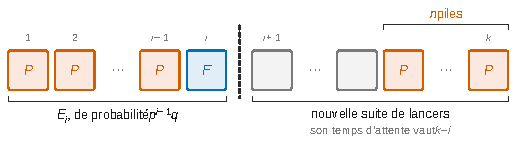
\includegraphics{figures/q30-frise-premier-face.pdf}
\caption*{Figure 3 --- Sur Eᵢ, le face du rang i coupe la suite des lancers : les
lancers i + 1, i + 2, \ldots{} forment une suite de même loi, dont le
temps d'attente vaut k − i quand Xₙ = k}
\end{figure}

La formule des probabilités totales donne
\equationajustee{\boxed{\begin{aligned}
\forall k>n,\quad P(X_n=k)&=qP(X_n=k-1)+qpP(X_n=k-2)\\
&\quad+\dots+qp^{n-1}P(X_n=k-n).
\end{aligned}}}

\hypertarget{question-31}{%
\subsection{Question 31}\label{question-31}}

Comme \(p\neq1\), \(\sum_{i=1}^np^{i-1}=\frac{1-p^n}{q}\), donc
\equationajustee{\boxed{\begin{aligned}
f(1)&=1-(1-p^n)\\
&=p^n>0.
\end{aligned}}}
La fonction \(f\) est polynomiale, donc continue en \(1\). Il existe ainsi \(\delta\in]0,1-p[\) tel que \(f>0\) sur \([1-\delta,1]\).

Le réel \(t=1-\frac\delta2\) vérifie \(p<1-\delta<t<1\) et \(f(t)>0\). \textbf{Il existe donc \(t\in]p,1[\) tel que \(f(t)\geqslant0\)}, c'est-à-dire
\equationajustee{q\sum_{i=1}^np^{i-1}t^{n-i}\leqslant t^n.\qquad(\ast)}

\begin{figure}[H]
\centering
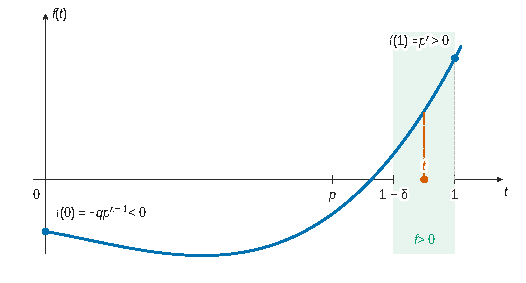
\includegraphics{figures/q31-allure-f.pdf}
\caption*{Figure 4 --- Allure de f, tracé pour n = 3 et p = 0,7 : f(1) = pⁿ
\textgreater{} 0, donc f \textgreater{} 0 sur un intervalle de la forme
1 − δ ≤ t ≤ 1, à droite de p, où l'on choisit t}
\end{figure}

\hypertarget{question-32}{%
\subsection{Question 32}\label{question-32}}

Récurrence forte sur \(k\in{\mathbb{N}}^*\).

\emph{Initialisation, \(1\leqslant k\leqslant n\).} Pour \(k<n\), on a \(P(X_n=k)=0\leqslant t^k\). Pour \(k=n\), on a \(P(X_n=n)=p^n\leqslant t^n\), car \(0<p<t\).

\emph{Hérédité.} Soit \(k>n\) tel que \(P(X_n=j)\leqslant t^j\) pour tout \(j\leqslant k-1\). Pour \(i\in\{1,\dots,n\}\), on a \(1\leqslant k-i\leqslant k-1\), donc par Q30 et \((\ast)\) :
\equationajustee{\begin{aligned}
P(X_n=k)&=\sum_{i=1}^nqp^{i-1}P(X_n=k-i)\\
&\leqslant\sum_{i=1}^nqp^{i-1}t^{k-i}\\
&=t^{k-n}\,q\sum_{i=1}^np^{i-1}t^{n-i}\\
&\leqslant t^{k-n}t^n\\
&=t^k.
\end{aligned}}
\equationajustee{\boxed{\forall k\in{\mathbb{N}}^*,\quad P(X_n=k)\leqslant t^k.}}

\hypertarget{question-33}{%
\subsection{Question 33}\label{question-33}}

\emph{Définition.} Soit \(|z|<1/t\). On a \(|P(X_n=k)z^k|\leqslant(t|z|)^k\), avec \(t|z|<1\).

La série \(\sum P(X_n=k)z^k\) converge donc absolument. \(G_{X_n}\) est ainsi définie sur le disque \(|z|<1/t\), de rayon \(\geqslant1/t>1\).

\emph{Calcul.} Notons \(u_k=P(X_n=k)\), \(G=G_{X_n}\), et soit \(|z|<1/t\).

On utilise Q29--Q30 et la convergence absolue : la famille \((qp^{i-1}u_{k-i}z^k)_{1\leqslant i\leqslant n,\ k>n}\) est sommable, majorée par \(q(t|z|)^{k-i}|z|^i\). Ainsi :
\equationajustee{\begin{aligned}
G(z)-p^nz^n&=\sum_{k>n}\sum_{i=1}^nqp^{i-1}u_{k-i}z^k\\
&=\sum_{i=1}^nqp^{i-1}z^i\sum_{j>n-i}u_jz^j\\
&=G(z)\,q\sum_{i=1}^np^{i-1}z^i,
\end{aligned}}
car \(u_j=0\) pour \(j<n\) et \(n-i<n\).

Comme \(|pz|<p/t<1\), on a \(q\sum_{i=1}^np^{i-1}z^i=qz\frac{1-p^nz^n}{1-pz}\). En multipliant par \(1-pz\) :
\equationajustee{G(z)\big[(1-pz)-qz+qp^nz^{n+1}\big]=p^nz^n(1-pz),}
soit
\equationajustee{G(z)\big(qp^nz^{n+1}-z+1\big)=p^nz^n(1-pz).}
Supposons que \(qp^nz^{n+1}-z+1\) s'annule en un \(z_0\) du disque. On aurait \(p^nz_0^n(1-pz_0)=0\), donc \(z_0=0\) (car \(pz_0\neq1\)).

Or ce facteur vaut \(1\) en \(0\). Donc
\equationajustee{\boxed{\forall z\in\mathbb{C},\ |z|<\frac1t,\quad G_{X_n}(z)=\frac{p^nz^n(1-pz)}{qp^nz^{n+1}-z+1}.}}
En particulier \(G_{X_n}(1)=\frac{p^nq}{qp^n}=1\), donc \(P(X_n=+\infty)=0\).

\hypertarget{question-34}{%
\subsection{Question 34}\label{question-34}}

Le rayon de convergence de \(\sum P(X_n=k)z^k\) est \(\geqslant1/t>1\). La série dérivée converge donc absolument en \(1\).

Ainsi \textbf{\(X_n\) (presque sûrement finie) admet une espérance}, et \(E(X_n)=G'_{X_n}(1)\).

Posons \(N(z)=p^n(z^n-pz^{n+1})\) et \(D(z)=1-z+qp^nz^{n+1}\). Alors :
\equationajustee{\begin{aligned}
N(1)&=qp^n,\\
D(1)&=qp^n,\\
N'(1)&=p^n\big(n-(n+1)p\big),\\
D'(1)&=(n+1)qp^n-1.
\end{aligned}}
Donc
\equationajustee{\begin{aligned}
E(X_n)&=\frac{N'(1)D(1)-N(1)D'(1)}{D(1)^2}\\
&=\frac{p^n\big(n-(n+1)p\big)-(n+1)qp^n+1}{qp^n}\\
&=\frac{p^n\big(n-(n+1)(p+q)\big)+1}{qp^n},
\end{aligned}}
\equationajustee{\boxed{\begin{aligned}
E(X_n)&=\frac{1-p^n}{qp^n}\\
&=\sum_{i=1}^n\frac1{p^i}.
\end{aligned}}}
Contrôles : pour \(n=1\), on retrouve \(\frac1p\). Pour \(n=2\), on retrouve \(\frac{1+p}{p^2}\).

\hypertarget{question-35}{%
\subsection{Question 35}\label{question-35}}

Soit \(i\in\{1,\dots,n\}\). Pour \(|z|<|\lambda_i|\), on a
\equationajustee{\begin{aligned}
\frac{a_i}{z-\lambda_i}&=-\frac{a_i}{\lambda_i}\cdot\frac{1}{1-z/\lambda_i}\\
&=-\sum_{k\geqslant0}\frac{a_i}{\lambda_i^{k+1}}z^k.
\end{aligned}}
Sur le disque \(|z|<\rho\), avec \(\rho=\min\left(\frac1t,|\lambda_1|,\dots,|\lambda_n|\right)\), on a donc
\equationajustee{\begin{aligned}
\sum_{k\geqslant1}P(X_n=k)z^k&=G_{X_n}(z)\\
&=\Big(a-\sum_{i=1}^n\frac{a_i}{\lambda_i}\Big)-\sum_{k\geqslant1}\Big(\sum_{i=1}^n\frac{a_i}{\lambda_i^{k+1}}\Big)z^k.
\end{aligned}}
Par unicité du développement en série entière sur un disque de rayon \(\rho>0\), pour tout \(k\in{\mathbb{N}}^*\) :
\equationajustee{\boxed{P(X_n=k)=-\sum_{1\leqslant i\leqslant n}\frac{a_i}{\lambda_i^{k+1}},}}
et de plus \(a=\sum_{i=1}^n\frac{a_i}{\lambda_i}\).

\hypertarget{d-obtenir-une-succession-de-pile-uxe0-la-suite-de-lancers-dune-piuxe8ce}{%
\section{D --- Obtenir une succession de pile à la suite de lancers d'une pièce}\label{d-obtenir-une-succession-de-pile-uxe0-la-suite-de-lancers-dune-piuxe8ce}}

\hypertarget{question-36}{%
\subsection{Question 36}\label{question-36}}

Si \(k<n\), \(A_{n,k}=\varnothing\) ; et \(A_{n,n}=P_1\cap\dots\cap P_n\) :
\equationajustee{\boxed{\begin{aligned}{}&\forall k\in\{1,\dots,n-1\},\ P(A_{n,k})=0,\\
&P(A_{n,n})=p^n.
\end{aligned}}}

\hypertarget{question-37}{%
\subsection{Question 37}\label{question-37}}

On reprend le système complet \((E_0,E_1,\dots,E_n)\) de Q30. Soit \(k>n\).

On a \(E_0\subset A_{n,k}\), donc \(P(E_0\cap A_{n,k})=p^n\).

Soit \(i\in\{1,\dots,n\}\). Sur \(E_i\), aucune série de \(n\) piles ne contient un lancer de rang \(\leqslant i\).

Ainsi \(A_{n,k}\) est réalisé si et seulement si les lancers de rangs \(i+1,\dots,k\) contiennent au moins \(n\) piles consécutifs. Ces \(k-i\) lancers sont indépendants, de même loi, et indépendants des \(i\) premiers.

Donc \(P(E_i\cap A_{n,k})=qp^{i-1}P(A_{n,k-i})\), avec \(k-i\geqslant1\).

Par la formule des probabilités totales :
\equationajustee{\boxed{\begin{aligned}
\forall k>n,\quad P(A_{n,k})&=p^n+qP(A_{n,k-1})+qpP(A_{n,k-2})\\
&\quad+\dots+qp^{n-1}P(A_{n,k-n}).
\end{aligned}}}

\hypertarget{question-38}{%
\subsection{Question 38}\label{question-38}}

\begin{lstlisting}[language=Python]
def probas_series(p, k, n):
    """Renvoie [P(A_{n,1}), ..., P(A_{n,k})] ; proba[j] contient P(A_{n,j+1})."""
    q = 1 - p
    proba = []
    for l in range(1, k + 1):
        if l < n:
            proba.append(0)
        elif l == n:
            proba.append(p ** n)
        else:
            s = p ** n
            for i in range(1, n + 1):
                s = s + q * p ** (i - 1) * proba[l - i - 1]   # P(A_{n,l-i})
            proba.append(s)
    return proba
\end{lstlisting}

Soit \(l>n\). Pour \(1\leqslant i\leqslant n\), on a
\equationajustee{0\leqslant l-n-1\leqslant l-i-1\leqslant l-2,}
donc les valeurs utilisées sont déjà calculées.

Coût : \(O(nk)\) opérations. Par exemple \texttt{probas\_series(\allowbreak{}0.5,\allowbreak{}\ 100,\allowbreak{}\ 5)\allowbreak{}{[}-1{]}\allowbreak{}} vaut environ \(0{,}8101\).

\hypertarget{question-39}{%
\subsection{Question 39}\label{question-39}}

Une suite constante \(v\) convient si et seulement si
\equationajustee{\begin{aligned}
v&=p^n+v\,q\sum_{i=1}^np^{i-1}\\
&=p^n+v(1-p^n),
\end{aligned}}
c'est-à-dire \(vp^n=p^n\), soit \(v=1\) :
\equationajustee{\boxed{\forall k\in{\mathbb{N}}^*,\ v_k=1.}}

\hypertarget{question-40}{%
\subsection{Question 40}\label{question-40}}

Posons \(w_k=1-P(A_{n,k})\). Pour \(k>n\), par Q37 et \(q\sum_{i=1}^np^{i-1}=1-p^n\) :
\equationajustee{\begin{aligned}
\sum_{i=1}^nqp^{i-1}w_{k-i}&=(1-p^n)-\sum_{i=1}^nqp^{i-1}P(A_{n,k-i})\\
&=(1-p^n)-\big(P(A_{n,k})-p^n\big)\\
&=w_k.
\end{aligned}}
La suite \((w_k)\) vérifie donc la relation de \((\star)\). Ses premiers termes sont \(w_i=1-P(A_{n,i})\) pour \(i\leqslant n\) (Q36).

Par l'unicité admise, la suite \((u_k)\) associée à ces conditions initiales est \((w_k)\). D'où \(P(A_{n,k})=1-u_k\) pour tout \(k\), avec
\equationajustee{\boxed{(b_1,\dots,b_{n-1},b_n)=(1,\dots,1,\ 1-p^n).}}

\hypertarget{question-41}{%
\subsection{Question 41}\label{question-41}}

D'après Q40, \(u_k=1-P(A_{n,k})=P\big(\overline{A_{n,k}}\big)\).
- Une série présente dans les \(k\) premiers lancers l'est dans les \(k+1\) premiers, donc \(A_{n,k}\subset A_{n,k+1}\). Ainsi \(P(A_{n,k})\leqslant P(A_{n,k+1})\) : \textbf{\((u_k)\) est décroissante}.
- L'événement \(\overline{A_{n,k}}\) contient \(F_1\cap\dots\cap F_k\), de probabilité \(q^k>0\). Donc \(u_k>0\).
- Soit \(k\geqslant n\). On a \(A_{n,n}\subset A_{n,k}\), donc \(P(A_{n,k})\geqslant p^n>0\). Ainsi \(u_k\leqslant1-p^n<1\).

\equationajustee{\boxed{\begin{aligned}{}&\forall k\geqslant n,\ 0<u_k<1,\\
&(u_k)_{k\in{\mathbb{N}}^*}\text{ \text{décroissante}}.
\end{aligned}}}

\hypertarget{question-42}{%
\subsection{Question 42}\label{question-42}}

\emph{\(M<1\).} Soit \(i\in\{n,\dots,2n-1\}\). Notons \(B_i\) l'événement « les lancers \(1,\dots,i+1-n\) donnent face et les lancers \(i+2-n,\dots,i+1\) donnent pile ».

Il est bien défini car \(i+1-n\geqslant1\). Les \(n\) derniers des \(i+1\) premiers lancers sont piles, donc \(B_i\subset A_{n,i+1}\).

Les \(i\) premiers lancers ne contiennent que \(n-1\) piles, consécutifs à la fin, donc \(B_i\subset\overline{A_{n,i}}\). Ainsi
\equationajustee{\begin{aligned}
u_i-u_{i+1}&=P(A_{n,i+1})-P(A_{n,i})\\
&\geqslant P(B_i)\\
&=q^{i+1-n}p^n>0.
\end{aligned}}
Comme \(u_i>0\), on en déduit \(\frac{u_{i+1}}{u_i}<1\). Un maximum d'un nombre fini de réels \(<1\) est \(<1\) : \(0<M<1\).

\emph{Choix de \(\alpha\).} On a \(f(1)=p^n>0\) et \(f\) est continue.

Il existe donc \(\delta\in]0,1[\) tel que \(f\geqslant0\) sur \([1-\delta,1]\). Posons \(\alpha=\max(M,1-\delta)\in[M,1[\).

Alors \(f(\alpha)\geqslant0\), soit
\equationajustee{q\sum_{i=1}^np^{i-1}\alpha^{n-i}\leqslant\alpha^n.\qquad(\ast\ast)}

\emph{Récurrence d'ordre \(n\) à partir du rang \(n+1\).} Montrons \(u_k\leqslant\alpha^{k-n}\) pour \(k\geqslant n+1\).

\emph{Rangs \(n+1\) à \(2n\).} Pour \(i\in\{n,\dots,2n-1\}\), on a \(u_{i+1}\leqslant Mu_i\leqslant\alpha u_i\).

Comme \(u_n=1-p^n<1\), on en déduit, pour \(1\leqslant j\leqslant n\), \(u_{n+j}\leqslant\alpha^ju_n\leqslant\alpha^j\).

\emph{Hérédité.} Soit \(k\geqslant2n+1\) tel que la propriété soit vraie aux rangs \(k-n,\dots,k-1\), tous \(\geqslant n+1\). Par \((\star)\) et \((\ast\ast)\) :
\equationajustee{\begin{aligned}
u_k&=\sum_{i=1}^nqp^{i-1}u_{k-i}\\
&\leqslant\sum_{i=1}^nqp^{i-1}\alpha^{k-i-n}\\
&=\alpha^{k-2n}\,q\sum_{i=1}^np^{i-1}\alpha^{n-i}\\
&\leqslant\alpha^{k-2n}\alpha^n\\
&=\alpha^{k-n}.
\end{aligned}}

\equationajustee{\boxed{\exists\alpha\in[M,1[,\ \forall k\geqslant n+1,\quad u_k\leqslant\alpha^{k-n}.}}

\hypertarget{question-43}{%
\subsection{Question 43}\label{question-43}}

La suite \((A_{n,k})_k\) est croissante pour l'inclusion. Par Q42, \(0<u_k\leqslant\alpha^{k-n}\to0\) puisque \(0\leqslant\alpha<1\). Par continuité croissante :
\equationajustee{\boxed{\begin{aligned}
P\Big(\bigcup_{k=1}^{+\infty}A_{n,k}\Big)&=\lim_{k\to+\infty}P(A_{n,k})\\
&=1-\lim_{k\to+\infty}u_k\\
&=1.
\end{aligned}}}
Prenons \(n=10\,000\). L'événement « on obtient à un moment une série d'au moins \(10\,000\) piles consécutifs » est exactement \(\bigcup_kA_{10\,000,k}\), car une telle série se termine à un rang fini \(k\).

Il est de probabilité \(1\) : il est presque sûr, quel que soit \(p\in]0,1[\).

\hypertarget{question-44}{%
\subsection{Question 44}\label{question-44}}

Ici \(n=5\), \(p=\frac12\), \(k=100\geqslant n+1\). Avec la valeur admise \(\alpha=0{,}9827\), Q42 donne \(u_{100}\leqslant\alpha^{95}\leqslant0{,}193\), d'où par Q40
\equationajustee{\boxed{\begin{aligned}
P(A_{5,100})&=1-u_{100}\\
&\geqslant1-0{,}193\\
&=0{,}807\geqslant0{,}8.
\end{aligned}}}
La probabilité d'obtenir au moins cinq piles consécutifs en \(100\) lancers d'une pièce équilibrée est donc au moins \(0{,}8\).

\emph{Remarque sur la donnée.} La valeur admise n'est pas compatible avec Q42. En effet, \(u_5=\frac{31}{32}\) et \(u_6=\frac{61}{64}\), donc
\equationajustee{M\geqslant\frac{u_6}{u_5}=\frac{61}{62}\approx0{,}9839>0{,}9827.}
De plus \(f(0{,}9827)<0\). Avec ce \(\alpha\), la majoration \(u_k\leqslant\alpha^{k-5}\) est d'ailleurs fausse à partir de \(k=113\).

Elle est cependant vraie pour \(k=100\) : la récurrence de Q37 donne \(u_{100}\approx0{,}1899\). La conclusion est donc exacte : \(P(A_{5,100})\approx0{,}8101\).

\hypertarget{question-45}{%
\subsection{Question 45}\label{question-45}}

Démarche, calquée sur la partie B.

\textbf{1. Linéariser.} Travailler sur \(u_k=1-P(A_{n,k})\), qui vérifie la récurrence linéaire d'ordre \(n\) \((\star)\) (Q40), sans terme constant.

\textbf{2. Vectoriser.} Poser \(V_k=(u_{k+n-1},\dots,u_{k+1},u_k)^\top\). Alors \(V_{k+1}=NV_k\), donc \(V_k=N^{k-1}V_1\). Ici \(N\) est la matrice compagnon de première ligne \((q,\ qp,\ \dots,\ qp^{n-1})\), de sous-diagonale formée de \(1\) et nulle ailleurs.

\textbf{3. Polynôme caractéristique.} Comme en Q17, \(\chi_N(X)=X^n-q\sum_{i=1}^np^{i-1}X^{n-i}\) : c'est le polynôme qui définit \(f\).

\textbf{4. Racines de module \(<1\).} Soit \(\mu\) une racine telle que \(|\mu|\geqslant1\). Alors
\equationajustee{\begin{aligned}
|\mu|^n&\leqslant q\sum_{i=1}^np^{i-1}|\mu|^{n-i}\\
&\leqslant|\mu|^{n-1}(1-p^n)\\
&<|\mu|^{n-1},
\end{aligned}}
d'où \(|\mu|<1\) : absurde. Les racines vérifient aussi \(\mu\neq0\), car \(\chi_N(0)=-qp^{n-1}\neq0\).

\textbf{5. Racines simples, diagonalisation.} Comme en Q19, on pose
\equationajustee{\Psi=(X-p)\chi_N=X^{n+1}-X^n+qp^n,}
de dérivée \(\Psi'=X^{n-1}\big((n+1)X-n\big)\).

Une racine multiple de \(\chi_N\) serait racine multiple de \(\Psi\), donc égale à \(\frac{n}{n+1}\).

On montre alors que cela force \(p=\frac n{n+1}\), et que \(p\) serait racine au moins triple de \(\Psi\). C'est exclu, car \(\Psi''(\frac n{n+1})\neq0\).

Donc \(\chi_N\) a \(n\) racines distinctes \(\mu_1,\dots,\mu_n\). On a alors \(N=QDQ^{-1}\), avec \(D=\mathrm{diag}(\mu_1,\dots,\mu_n)\).

\textbf{6. Conclure.} Comme en Q21, la dernière composante de \(V_k=QD^{k-1}Q^{-1}V_1\) s'écrit \(u_k=\sum_i\gamma_i\mu_i^{k-1}\). On pose \(c_i=\gamma_i/\mu_i\) :
\equationajustee{\boxed{\begin{aligned}{}&\forall k\in{\mathbb{N}}^*,\ P(A_{n,k})=1-\sum_{i=1}^nc_i\mu_i^k,\\
&|\mu_i|<1.
\end{aligned}}}
Les \(c_i\) se déterminent, si on le souhaite, par les \(n\) conditions initiales (système de Vandermonde inversible puisque les \(\mu_i\) sont distincts et non nuls).

\end{document}
